% ============================================================================
%  DSA5208 Final Project report.  Build locally:  cd report && tectonic report.tex
%  Narrative flow (Spark-report style); rubric coverage tagged in comments so it
%  can be audited at a glance (tags do NOT render in the PDF):
%    [R1 5pt] explain algorithm         -> Sec 2
%    [R2 5pt] serial scaling, vary N&F  -> Sec 5
%    [R3 10pt] MPI strong+weak >=256,    -> Sec 6
%              speedup/eff, communication
%    [R4 10pt] MPI+X (OpenMP) + GPU      -> Sec 7
%    [R5 5pt] overall discussion         -> Sec 8
%  General instructions also require: validation (Sec 4), machine stated on
%  figures (Sec 3/6), real-data conclusions (Sec 8), AI usage (Sec 9), authors +
%  code link (title).
% ============================================================================
\documentclass[11pt]{article}
\usepackage[margin=1in]{geometry}
\usepackage{graphicx}
\usepackage{amsmath}
\usepackage{booktabs}
\usepackage{siunitx}
\usepackage{listings}
\usepackage{xcolor}
\usepackage{hyperref}
\usepackage{parskip}
\usepackage{float}
\widowpenalty=10000
\clubpenalty=10000
\hypersetup{colorlinks=true, urlcolor=blue, linkcolor=black}
\graphicspath{{../results/report_assets/}{../results/report_assets_vanda_1537141/}{figures/}{../figures/}}
\lstset{basicstyle=\ttfamily\small,breaklines=true,frame=single}

\title{A Hybrid-Parallel Decision Tree:\\ MPI, OpenMP and CUDA Scaling of Histogram-Based CART}
\author{Jen-Chien Huang (A0353871) \and Bing Wen Lim \and Haoran Zhang}
\date{\href{https://github.com/dannyhuang1111/dsa5208-distributed-decision-tree}{\texttt{https://github.com/dannyhuang1111/dsa5208-distributed-decision-tree}}}

\begin{document}
\maketitle

% ===========================================================================
\section{Introduction}

A decision tree is built greedily: starting from all the training rows at the root, each node chooses the one feature and threshold that best separates the two classes, splits its rows accordingly, and repeats on the two children until a stopping rule fires. This project parallelizes the \emph{construction} of a binary classification tree and studies how different parallelization choices affect its scaling and efficiency.

The problem is a good parallelization target because it is \emph{not} embarrassingly parallel. Although the training rows can be partitioned across processes trivially, choosing a split needs the class counts on both sides of every candidate threshold \emph{summed over all rows}. With the rows spread across processes, no process can decide a split alone: each node forces a collective communication, and the children a node produces determine the work of the next level. That per-node global reduction, and the dependency between levels, are the source of the communication and load-balancing challenges we examine.

The report follows the project from the algorithm and its serial cost model (Sections~\ref{sec:algo}--\ref{sec:design}), through a correctness validation (Section~\ref{sec:valid}), to the three scaling studies: serial problem-size scaling (Section~\ref{sec:serial}), pure-MPI strong and weak scaling to \num{256} cores (Section~\ref{sec:mpi}), and the MPI+X results for the MPI+OpenMP hybrid and the CUDA GPU arm (Section~\ref{sec:mpix}). Reproduction instructions are in \texttt{README.md}.

% ===========================================================================
\section{The algorithm and the computing environment}\label{sec:algo}
% [R1 5pt] explain the algorithm being parallelized

\subsection{Histogram-based CART with the Gini criterion}

For a node holding $t$ samples of which $p$ are positive, the Gini impurity is
\begin{equation}
G(p,t) = 1 - \left(\tfrac{p}{t}\right)^2 - \left(\tfrac{t-p}{t}\right)^2 ,
\end{equation}
and a candidate split into a left child $(p_L,t_L)$ and right child $(p_R,t_R)$ is scored by the Gini gain
\begin{equation}
\Delta G = G(p,t) - \frac{t_L}{t}\,G(p_L,t_L) - \frac{t_R}{t}\,G(p_R,t_R).
  \label{eq:gain}
\end{equation}
The node adopts the (feature, threshold) with the largest $\Delta G$, and recursion stops when the node reaches the maximum depth, holds at most \texttt{min-split} samples, is pure, or no split gives positive gain.

Rather than sorting each feature at every node, we use a \textbf{histogram} formulation. Each feature's values are placed into bins; when a feature has at most \num{256} distinct values the bins are its exact distinct values, so the candidate thresholds are identical to a sort-based search. A node is then summarised by, per bin, the pair $[\text{count},\text{positive count}]$. Scanning those bins in order reproduces every candidate split from Equation~\ref{eq:gain}. The histogram is the unit of work that the parallelization distributes, and because its entries are integers, summing them across processes is exact and order-independent --- a property we rely on for both correctness and determinism (Sections~\ref{sec:design}--\ref{sec:valid}).

Per node, the dominant cost is building the histogram, which is $O(n_{\text{node}}\times F)$ for $n_{\text{node}}$ rows and $F$ features. Summed over the tree, training cost grows with both the number of rows $N$ and the number of features $F$; Section~\ref{sec:serial} measures both.

\subsection{One source, four configurations}

The algorithm is written once in \texttt{src/dt.cpp}; MPI and OpenMP are enabled by compile-time guards so the split-search logic is byte-identical in every build. This yields the four configurations the report compares:

\begin{itemize}
  \item \textbf{serial} --- no MPI, no OpenMP; the single-core baseline for speedup;
  \item \textbf{pure MPI} --- the MPI build run with \texttt{OMP\_NUM\_THREADS=1}, so MPI is the only parallelism (Section~\ref{sec:mpi});
  \item \textbf{MPI+OpenMP} --- the same build with multiple threads per rank (Section~\ref{sec:mpix});
  \item \textbf{CUDA} --- a separate GPU implementation of the histogram hot path (Section~\ref{sec:mpix}).
\end{itemize}

\subsection{Computing environment}
% general instruction: runtime figures from Atlas or Vanda -> state the machine

Benchmarks were run on the NUS \textbf{Vanda} HPC cluster. The \num{256}-core CPU scaling run recorded in \texttt{results/raw/env\_20261110\_224241\_1537141.txt} (PBS job \texttt{1537141.stdct-mgmt-02}, head compute node \texttt{CN-064}) used four dual-socket \textbf{Intel Xeon Platinum 8452Y} nodes (\num{36} cores per socket, \num{72} physical cores per node, one hardware thread per core, \num{64} cores allocated per node for \num{256} cores total), \textbf{OpenMPI 4.1.4}, and \textbf{GCC 12.2.0}; each benchmark point is the median of \num{3} repetitions after a warm-up tree. The GPU benchmarks (PBS jobs \texttt{1536934} and \texttt{1537453}) ran on a Vanda GPU node equipped with an \textbf{NVIDIA A40} (\SI{48}{GB} GDDR6, Ampere architecture) compiled with \textbf{CUDA 12.2}.

\subsection{Dataset}

We use the preprocessed Instacart reorder dataset \texttt{instacart\_clean.csv}: \num{200000} orders, \num{7} features (order number, day of week, hour of day, days since prior order, add-to-cart order, aisle id, department id) and a binary \texttt{reordered} label. The file is clean (no missing values) and every feature has at most \num{256} distinct values, so binning is exact. Plainly stated, the \texttt{instacart\_clean.csv} committed in the repository is the schema-matched sample generated by \texttt{preprocess.py} (which plants higher reorder probabilities for \texttt{add\_to\_cart\_order} $\le 3$ and \texttt{days\_since\_prior\_order} $= 7$ when the raw multi-gigabyte Kaggle CSVs are not present locally).

Because \num{200000} rows are far too few to occupy hundreds of cores --- the per-node reduction would dominate --- the scaling studies instead use a deterministic synthetic generator that reproduces the Instacart schema and value ranges. Row $r$ is a pure function of $(\text{seed},r)$, so the dataset is identical for every process count and nothing is read from disk, letting us vary $N$ and $F$ freely. The synthetic data is Instacart-\emph{like} in shape, not sampled from the real file; real-data conclusions (Section~\ref{sec:discuss}) come from \texttt{instacart\_clean.csv} itself.

% ===========================================================================
\section{Parallelization design}\label{sec:design}
% [R5 5pt] (how we chose to parallelize; which parts communicate most)
% general instruction: design decisions

\paragraph{Data parallelism over rows, not over tree nodes.}
The rows are block-distributed across processes once, at load time, and never move again. For each node, every process builds the histogram of \emph{its own} rows and a single \texttt{MPI\_Allreduce} with integer sum produces the global histogram; every process then scans that identical histogram and independently reaches the identical split, so no split decision needs to be broadcast.

We deliberately did not parallelize by handing whole subtrees to different processes (task parallelism). Near the root there are only a handful of nodes but the most data, so subtree parallelism is scarcest exactly where the cost is greatest; sibling subtrees are unbalanced, so processes would idle; and assigning a subtree to a process would require reshuffling rows at every split. Data parallelism instead keeps every process busy on every node and attacks the cost where it lives --- the histogram build, which Section~\ref{sec:mpi} shows dominates the runtime.

\paragraph{Determinism as a design constraint.}
Because the reduction sums integers, its result does not depend on the number of processes or the order of summation, so the tree is bit-for-bit identical across all configurations. This both gives a strong correctness check (Section~\ref{sec:valid}) and ruled out alternatives that would have broken it, such as reducing floating-point partial gains or assigning subtrees to processes.

\paragraph{Two communication patterns (tree growth).}
The same tree can be grown two ways, trading off message count against message size. \emph{Node-wise} growth is depth-first with one reduction per internal node (many small messages, latency-bound); \emph{level-wise} growth is breadth-first and reduces the stacked histograms of all nodes at one depth in a single collective (far fewer, larger messages). At depth \num{6} on $N=\num{32000000}, F=\num{28}$ (Table~\ref{tab:design} and Figure~\ref{fig:design}), node-wise growth issues \num{64} \texttt{MPI\_Allreduce} calls whereas level-wise issues only \num{7}, while both exchange the exact same total payload (\SI{0.6955}{MB}). Eliminating \num{57} collective round-trips reduces training time at \num{256} cores from \SI{0.1733}{s} to \SI{0.0634}{s} for $64\times 4$ (\num{2.73}$\times$ faster) and from \SI{0.1075}{s} to \SI{0.0652}{s} for $256\times 1$ (\num{1.65}$\times$ faster).

\paragraph{Two OpenMP strategies (X = OpenMP).}
Within a rank, threads can either split the \emph{rows} (each thread fills a private histogram, then a parallel reduction combines them) or split the \emph{features} (threads share one histogram, with parallelism capped by $F$). As Table~\ref{tab:design} confirms, splitting rows (\texttt{sample}) beats splitting features (\texttt{feature}) across every configuration: at $64\times 4$ with level-wise growth, \texttt{sample} runs in \SI{0.0634}{s} versus \SI{0.1530}{s} for \texttt{feature} (\num{2.41}$\times$ faster), because row parallelism scales with $N/p$ rather than being bottlenecked by $F=\num{28}$.

\begin{table}[H]
\centering
\caption{Design-choice comparison at \num{256} cores ($N=\num{32000000}, F=\num{28}$, depth \num{6}; from \texttt{design\_20261110\_224241\_1537141.csv}).}
\label{tab:design}
\begin{tabular}{rrrrrr}
\toprule
Ranks & Threads & Growth & OpenMP & \texttt{Allreduce} calls & Median time (s) \\
\midrule
64  & 4 & level & sample  &  7 & \textbf{0.0634} \\
64  & 4 & level & feature &  7 & 0.1530 \\
64  & 4 & node  & sample  & 64 & 0.1733 \\
64  & 4 & node  & feature & 64 & 0.2740 \\
256 & 1 & level & sample  &  7 & \textbf{0.0652} \\
256 & 1 & level & feature &  7 & 0.0806 \\
256 & 1 & node  & sample  & 64 & 0.1075 \\
256 & 1 & node  & feature & 64 & 0.1161 \\
\bottomrule
\end{tabular}
\end{table}

\begin{figure}[H]
\centering
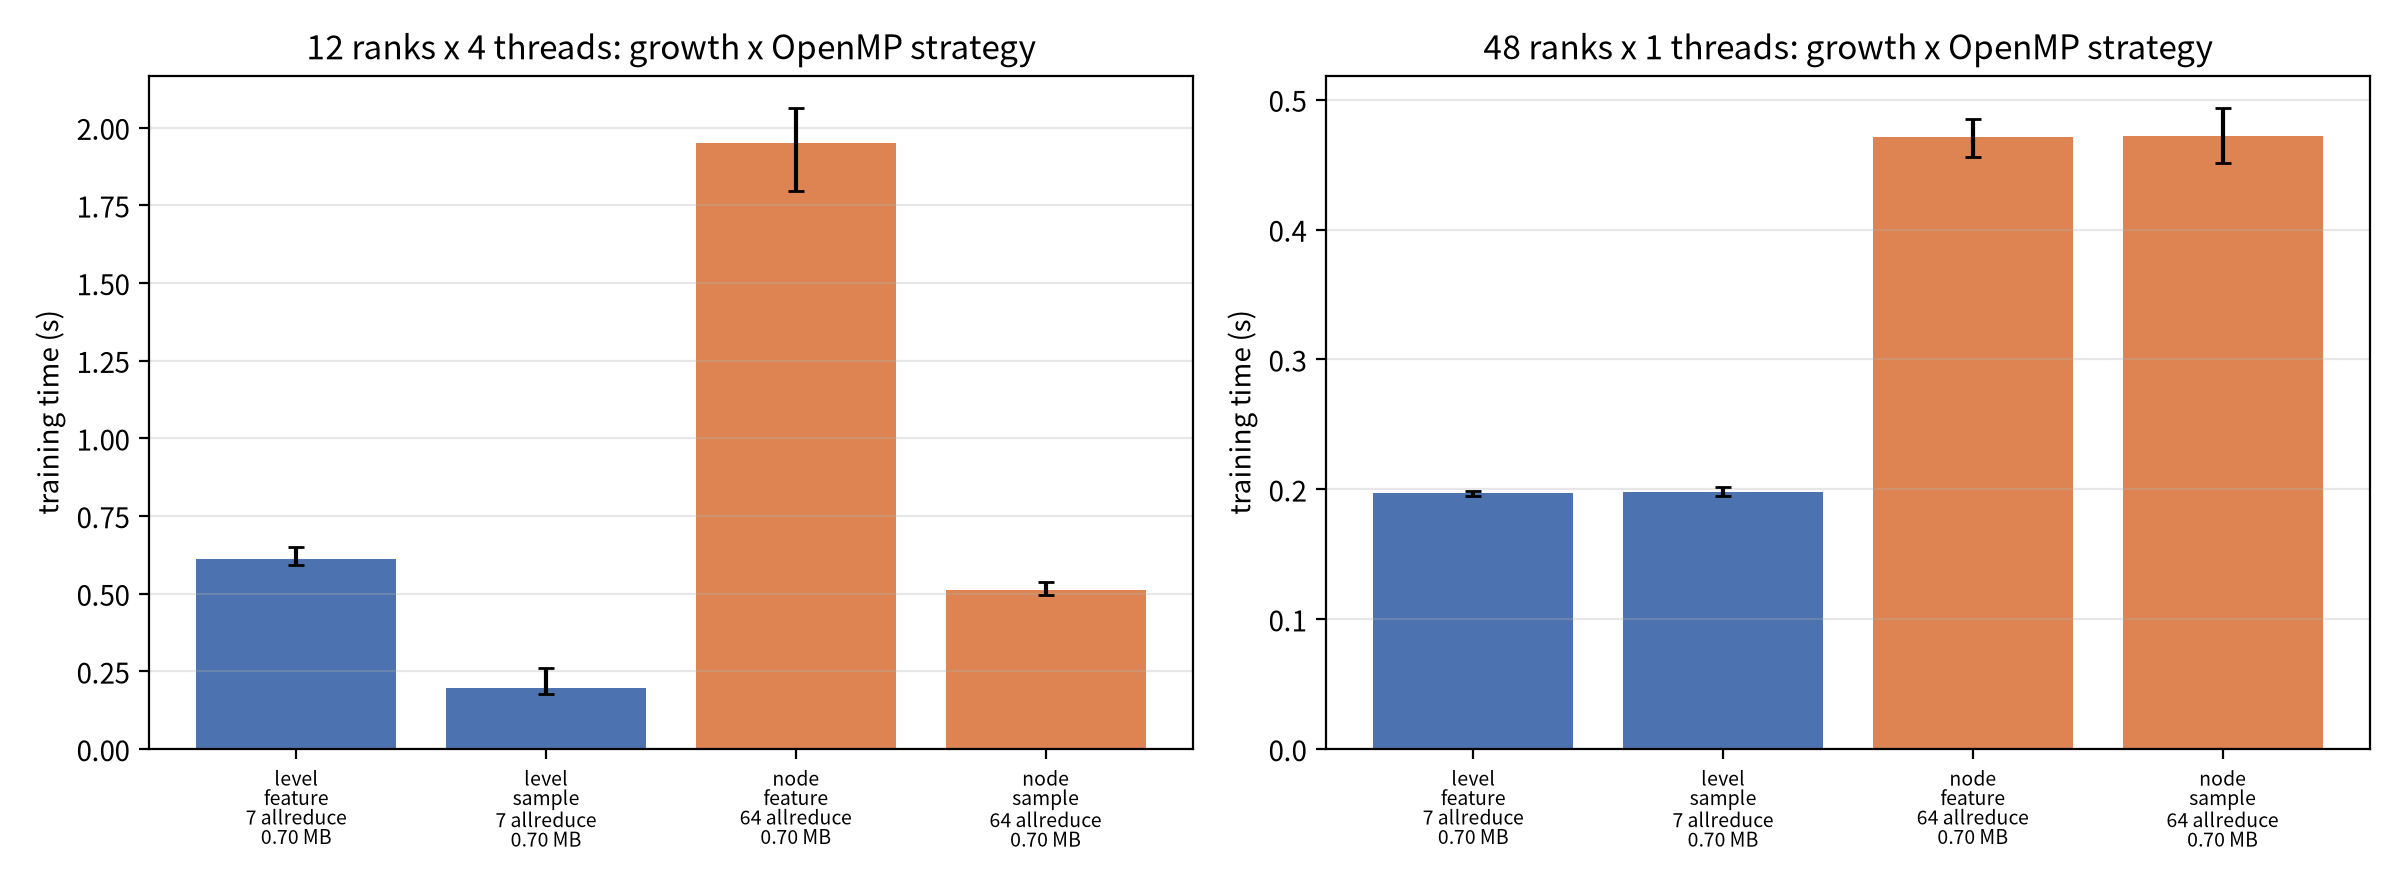
\includegraphics[width=0.75\linewidth]{design_choices.png}
\caption{Level-wise vs.\ node-wise growth and sample vs.\ feature OpenMP strategies on Vanda (\num{256} cores, $N=\num{32000000}, F=\num{28}$).}
\label{fig:design}
\end{figure}

% ===========================================================================
\section{Validating correctness}\label{sec:valid}
% general instruction: validation that the parallel algorithm works correctly

Two independent checks establish that the parallel builds compute the right tree.

First, \textbf{cross-configuration equivalence} exploits the determinism above. The script \texttt{scripts/check\_equivalence.sh} hashes the entire tree (structure, split features, thresholds and leaf predictions) with FNV-1a and requires every configuration --- process counts $\{1,2,3,4,7\}$, thread counts $\{1,2,3\}$, both growth modes, both OpenMP strategies, both the synthetic and CSV input paths, on a prime number of rows ($N=\num{100003}$) so the row blocks are uneven --- to reproduce the serial reference hash (\texttt{0bfc2e3832b96e3f}) exactly, reporting:
\begin{center}
\texttt{64 / 64 configurations identical to the reference}
\end{center}
In addition, \texttt{analysis/plot\_results.py} verifies tree hashes across all \num{969} benchmark runs in \texttt{results/raw/}: every $(N,F,\text{depth})$ dataset produces exactly \num{1} distinct tree hash across all \num{33} parallel configurations (e.g.\ hash \texttt{50e4598e0ff9ac07} across all \num{222} runs at $N=\num{32000000}, F=\num{28}$).

Second, an \textbf{external reference}: \texttt{scripts/compare\_sklearn.py} rebuilds the tree dumped by \texttt{dt --dump-tree} and compares it node by node against scikit-learn's \texttt{DecisionTreeClassifier} on \texttt{instacart\_clean.csv}. Both build a \num{125}-node tree with identical training accuracy (\SI{68.5035}{\percent}) and agree on \SI{99.9850}{\percent} of row predictions (\num{123} of \num{125} nodes match directly, with one exact-tie leaf accepted and a single bottom-level tie at \texttt{rootRLRRR} where $f_4 \le 5$ and $f_5 \le 4.5$ yield equal impurity gain).

This equivalence was also what motivated the current design. An earlier MPI implementation combined rank-local split gains with \texttt{MPI\_MAXLOC}, which is not the global Gini gain; its trees drifted with the process count (training accuracy \SI{68.46}{\percent} at one rank versus \SI{68.42}{\percent} at eight on the same \num{200000} rows), while the root split stayed correct and so hid the bug from shallow checks. The histogram-reduction design removes this drift completely.

% ===========================================================================
\section{Serial scaling with problem size}\label{sec:serial}
% [R2 5pt] serial runtime scaling, varying BOTH dimensions: N (rows) and F (features)

The serial build establishes both the speedup baseline and the cost model. We vary the two dimensions of problem size independently: the number of rows $N\in\{1,2,4,8,16,32\}\times 10^6$ at fixed $F=\num{28}$, and the number of features $F\in\{7,14,28,56,112,224\}$ at fixed $N=\num{8000000}$. Because per-node work is $O(n_{\text{node}}\times F)$, both should give near-linear runtime growth.

\begin{table}[H]
\centering
\caption{Serial runtime sweep varying $N$ at $F=\num{28}$ (left) and varying $F$ at $N=\num{8000000}$ (right) on one Xeon Platinum 8452Y core (\texttt{serial\_scan\_20261110\_224241\_1537141.csv}).}
\label{tab:serial}
\begin{tabular}{rr@{\hspace{2.5em}}rr}
\toprule
Rows $N$ ($F=28$) & Median $T_1$ (s) & Features $F$ ($N=8\text{M}$) & Median $T_1$ (s) \\
\midrule
 \num{1000000} & 0.2392 &   7 &  0.4669 \\
 \num{2000000} & 0.2998 &  14 &  0.7027 \\
 \num{4000000} & 0.6080 &  28 &  1.2012 \\
 \num{8000000} & 1.2012 &  56 &  2.3235 \\
\num{16000000} & 2.5358 & 112 &  4.7411 \\
\num{32000000} & 4.8806 & 224 & 10.5904 \\
\bottomrule
\end{tabular}
\end{table}

\begin{figure}[H]
\centering
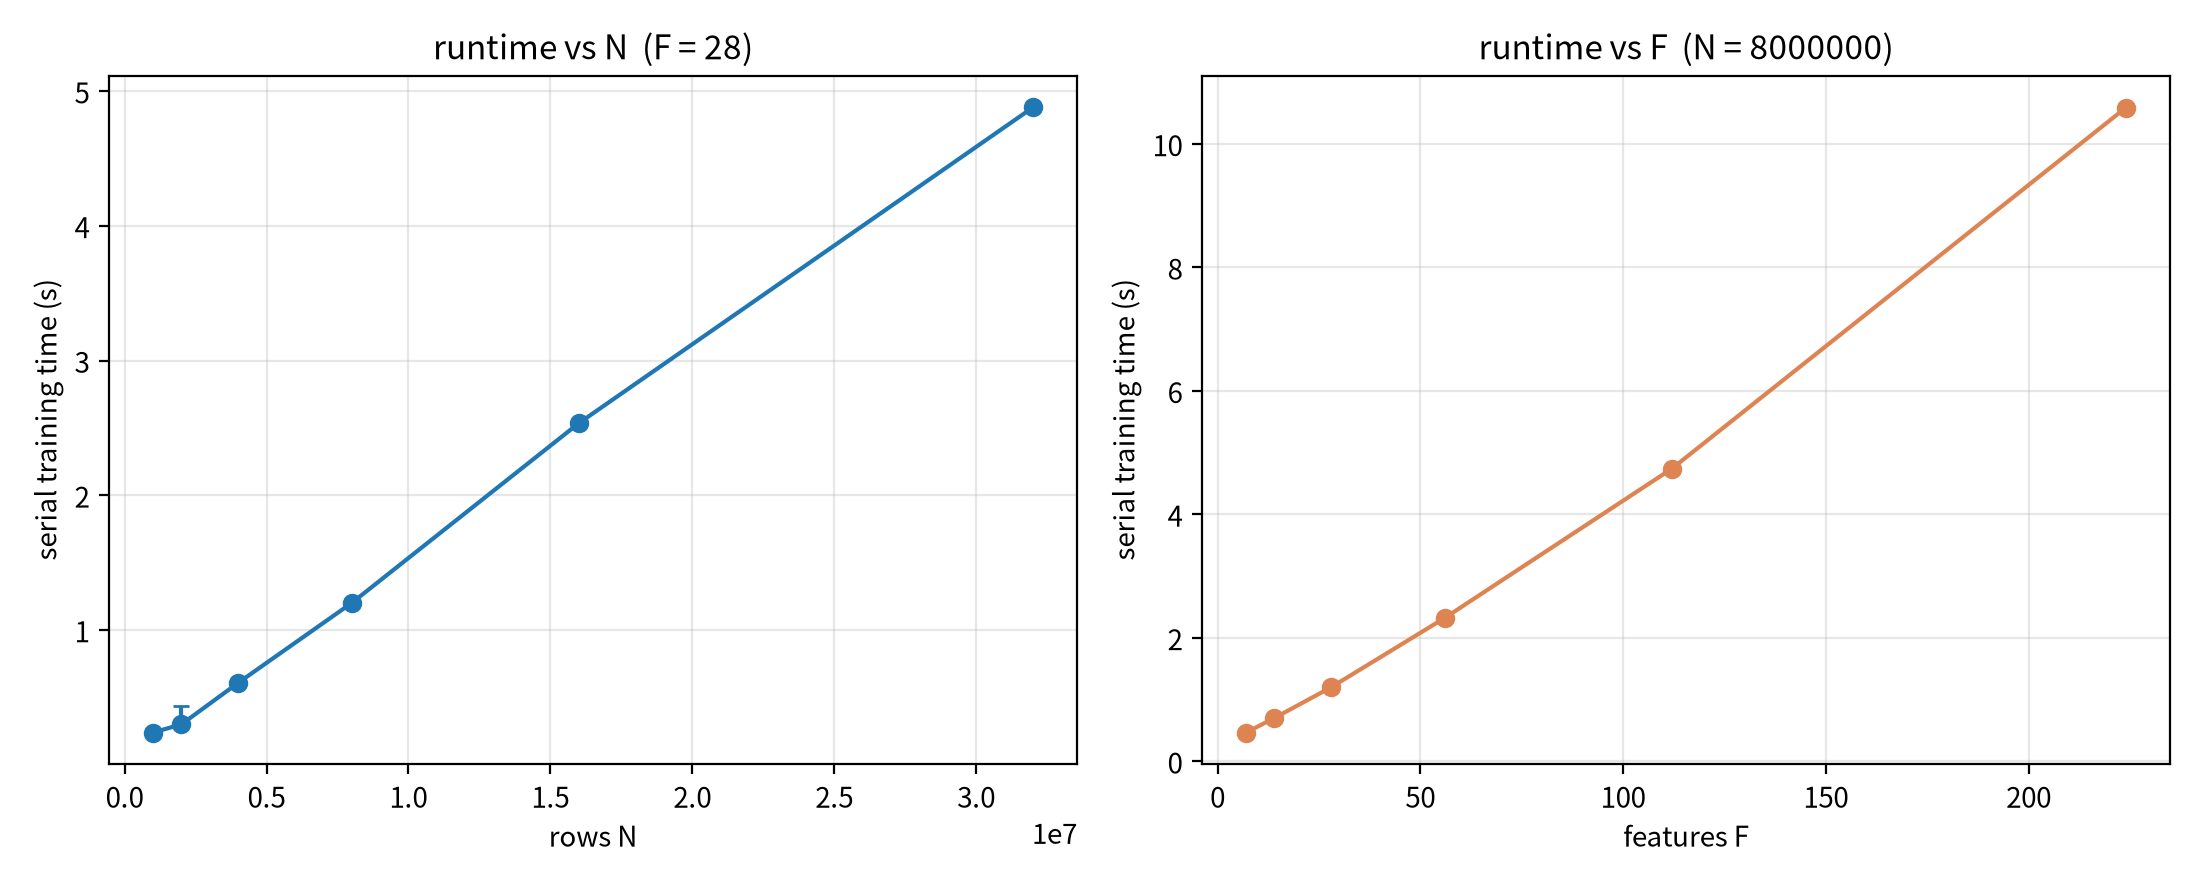
\includegraphics[width=\linewidth]{serial_scan.png}
\caption{Serial training time vs.\ rows $N$ at $F=\num{28}$ (left) and vs.\ features $F$ at $N=\num{8000000}$ (right) on Vanda.}
\label{fig:serial}
\end{figure}

Table~\ref{tab:serial} and Figure~\ref{fig:serial} confirm the $O(N\times F)$ cost model along both axes. Doubling $N$ from \num{4}M to \num{32}M at $F=\num{28}$ scales runtime linearly with a constant slope of \SI{0.152}{\micro\second} per row ($\num{32}\text{M}/\num{4}\text{M}=8\times$ data gives $\num{4.881}/\num{0.608}=\num{8.03}\times$ runtime). Likewise, doubling $F$ from \num{14} to \num{224} at $N=\num{8}M$ increases runtime from \SI{0.703}{s} to \SI{10.590}{s} ($\num{16}\times$ features gives $\num{15.07}\times$ runtime, slope $\approx \SI{0.046}{s}$ per feature).

% ===========================================================================
\section{Pure-MPI strong and weak scaling}\label{sec:mpi}
% [R3 10pt] strong + weak to >=256 cores; speedup + efficiency; communication impact

This section uses the pure-MPI configuration (one rank per core, \texttt{OMP\_NUM\_THREADS=1}), alongside the $4$-thread-per-rank hybrid curve for reference. Speedup is $S_p = T_1/T_p$ against the serial baseline on the same data, and parallel efficiency is $E_p = S_p/p$ for $p$ cores; $T_p$ is the maximum over ranks of the barrier-to-barrier training time.

\subsection{Strong scaling}

Here the problem is fixed at $N=\num{32000000}$ rows and the core count grows from \num{1} to \num{256} cores across four Vanda nodes ($F\in\{7,14,28,56\}$; we focus on $F=\num{28}$ in Table~\ref{tab:strong} and Figure~\ref{fig:strong}).

\begin{table}[H]
\centering
\caption{Strong scaling to \num{256} cores on Vanda ($N=\num{32000000}, F=\num{28}$, depth \num{6}, $T_{\text{serial}}=\SI{5.169}{s}$; from \texttt{strong\_scaling\_F28.csv}).}
\label{tab:strong}
\begin{tabular}{rrrrrr}
\toprule
Cores $p$ & Pure MPI $T_p$ (s) & Speedup $S_p$ & Efficiency $E_p$ & Hybrid ($t=4$) $T_p$ (s) & Hybrid $S_p$ \\
\midrule
  1 & 5.353 &  0.97$\times$ & 96.6\% &    --- &    --- \\
  2 & 2.972 &  1.74$\times$ & 87.0\% &    --- &    --- \\
  4 & 1.412 &  3.66$\times$ & 91.5\% & 1.405  &  3.68$\times$ \\
  8 & 0.945 &  5.47$\times$ & 68.4\% & 0.902  &  5.73$\times$ \\
 16 & 0.420 & 12.31$\times$ & 76.9\% & 0.523  &  9.89$\times$ \\
 32 & 0.293 & 17.67$\times$ & 55.2\% & 0.349  & 14.80$\times$ \\
 64 & 0.202 & 25.64$\times$ & 40.1\% & 0.187  & 27.61$\times$ \\
128 & 0.102 & 50.76$\times$ & 39.7\% & 0.117  & 44.32$\times$ \\
256 & \textbf{0.0684} & \textbf{75.54$\times$} & \textbf{29.5\%} & \textbf{0.0717} & \textbf{72.10$\times$} \\
\bottomrule
\end{tabular}
\end{table}

\begin{figure}[H]
\centering
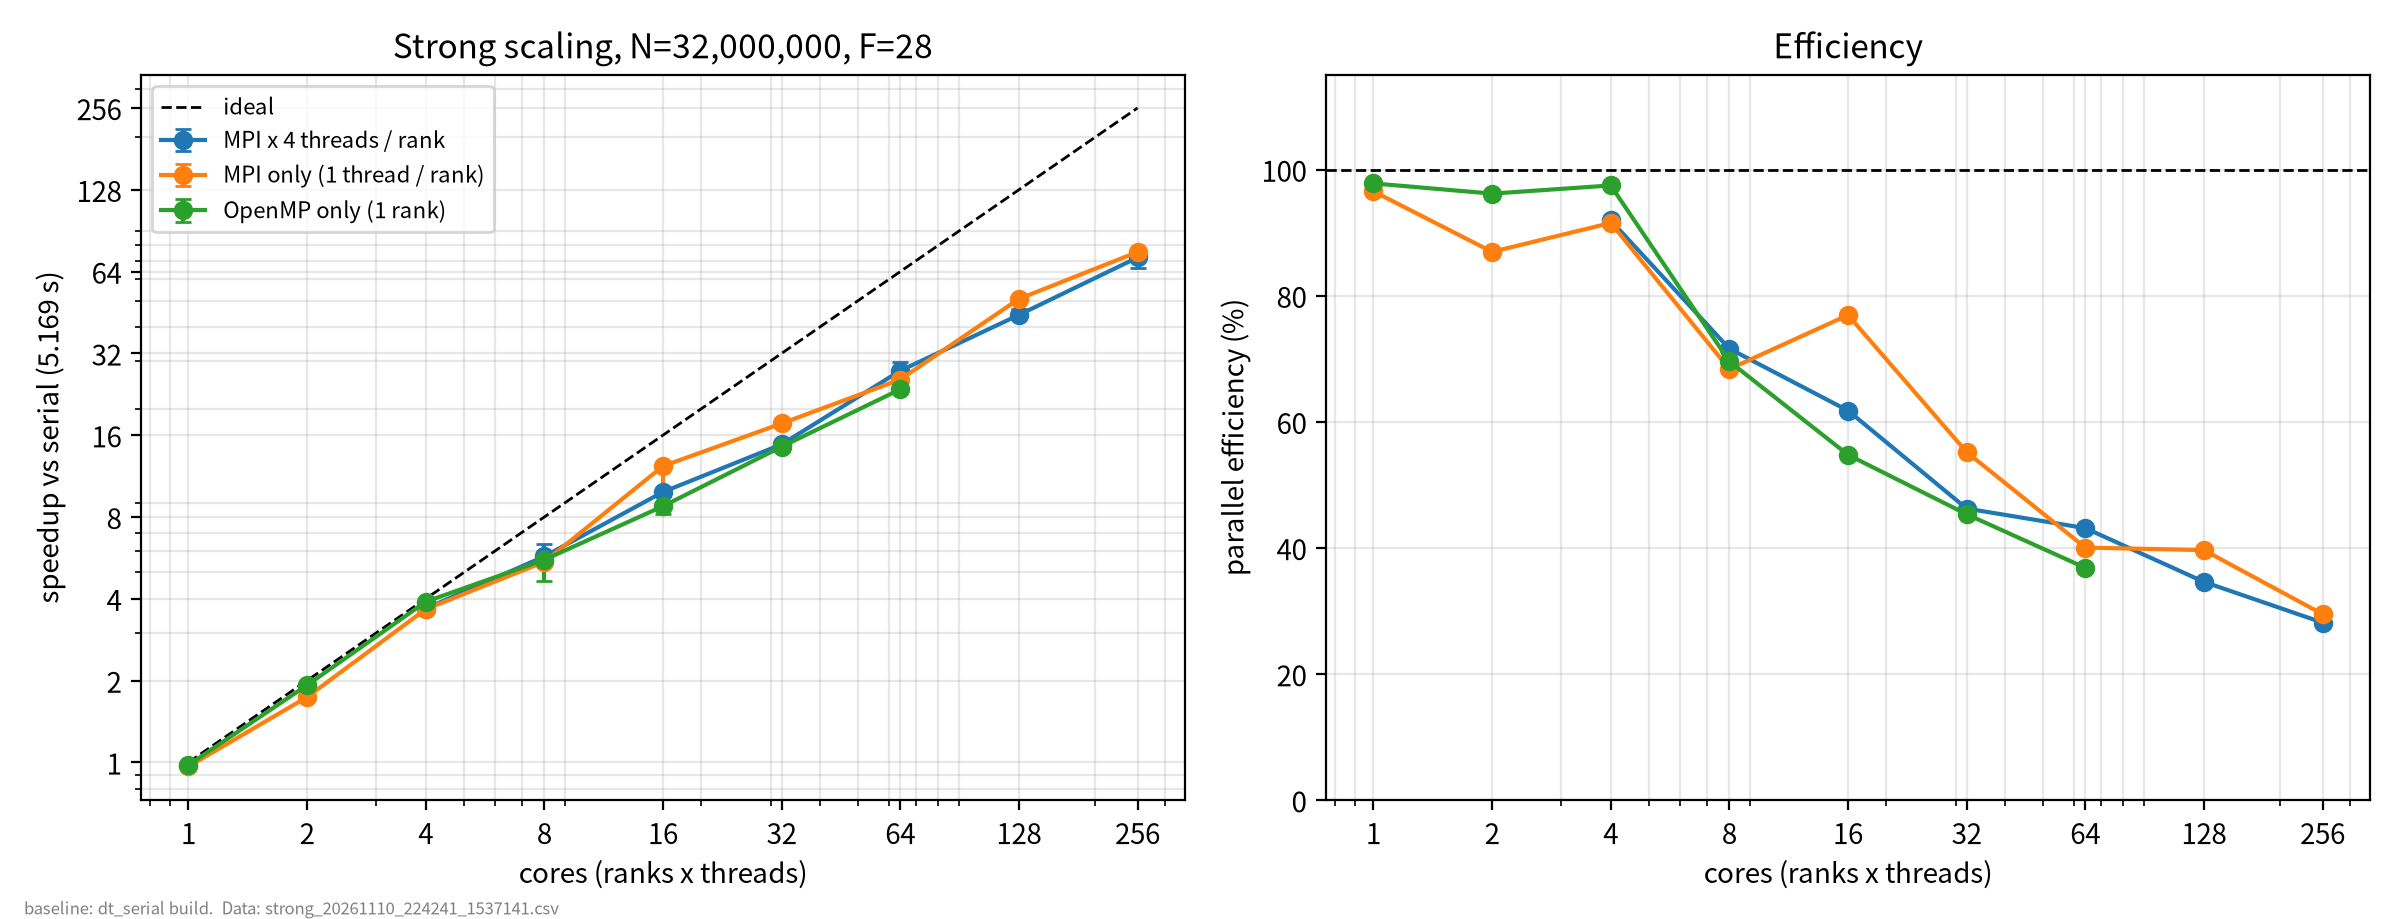
\includegraphics[width=\linewidth]{strong_scaling_F28.png}
\caption{Strong scaling speedup (left) and parallel efficiency (right) to \num{256} cores on Vanda ($N=\num{32000000}, F=\num{28}$).}
\label{fig:strong}
\end{figure}

Pure MPI reduces training time from \SI{5.169}{s} to \SI{0.0684}{s} at \num{256} cores (\num{75.54}$\times$ speedup, \SI{29.5}{\percent} efficiency), while the $64\times 4$ hybrid reaches \SI{0.0717}{s} (\num{72.10}$\times$). Across the feature sweep at \num{256} cores, pure-MPI speedup increases with $F$: \num{71.33}$\times$ at $F=7$, \num{56.06}$\times$ at $F=14$, \num{75.54}$\times$ at $F=28$, and \textbf{\num{95.34}$\times$} (\SI{37.2}{\percent} efficiency, \SI{9.885}{s} down to \SI{0.1037}{s}) at $F=56$. Efficiency stays above \SI{75}{\percent} up to \num{16} cores, steps down at \num{32}--\num{64} cores as a single node's memory channels saturate, and tapers to \SI{29.5}{\percent} at \num{256} cores once per-rank histogram work shrinks to $\sim\SI{40}{ms}$ and multi-node \texttt{MPI\_Allreduce} latency becomes a larger fraction of total time.

\subsection{Weak scaling}

Here the work per core is fixed at \num{1000000} rows per core and both $N$ and $p$ grow together from $N=\num{1000000}$ ($p=1$) to $N=\num{256000000}$ ($p=256$).

\begin{table}[H]
\centering
\caption{Weak scaling to \num{256} cores / \num{256}M rows at \num{1}M rows per core ($F=\num{28}$, depth \num{6}; from \texttt{weak\_scaling.csv}).}
\label{tab:weak}
\begin{tabular}{rrrrrr}
\toprule
Cores $p$ & Total rows $N$ & Pure MPI $T_p$ (s) & Weak $E_p$ & Hybrid ($t=4$) $T_p$ (s) & Hybrid $E_p$ \\
\midrule
  1 &   \num{1000000} & 0.2563 & 100.0\% &    --- &    --- \\
  2 &   \num{2000000} & 0.2546 & 100.7\% &    --- &    --- \\
  4 &   \num{4000000} & 0.2720 &  94.2\% & 0.2523 & 100.0\% \\
  8 &   \num{8000000} & 0.3159 &  81.1\% & 0.2662 &  94.8\% \\
 16 &  \num{16000000} & 0.3410 &  75.2\% & 0.2896 &  87.1\% \\
 32 &  \num{32000000} & 0.3532 &  72.6\% & 0.4003 &  63.0\% \\
 64 &  \num{64000000} & 0.4296 &  59.7\% & 0.4013 &  62.9\% \\
128 & \num{128000000} & 0.4928 &  52.0\% & 0.4235 &  59.6\% \\
256 & \num{256000000} & \textbf{0.4863} & \textbf{52.7\%} & \textbf{0.5884} & \textbf{42.9\%} \\
\bottomrule
\end{tabular}
\end{table}

\begin{figure}[H]
\centering
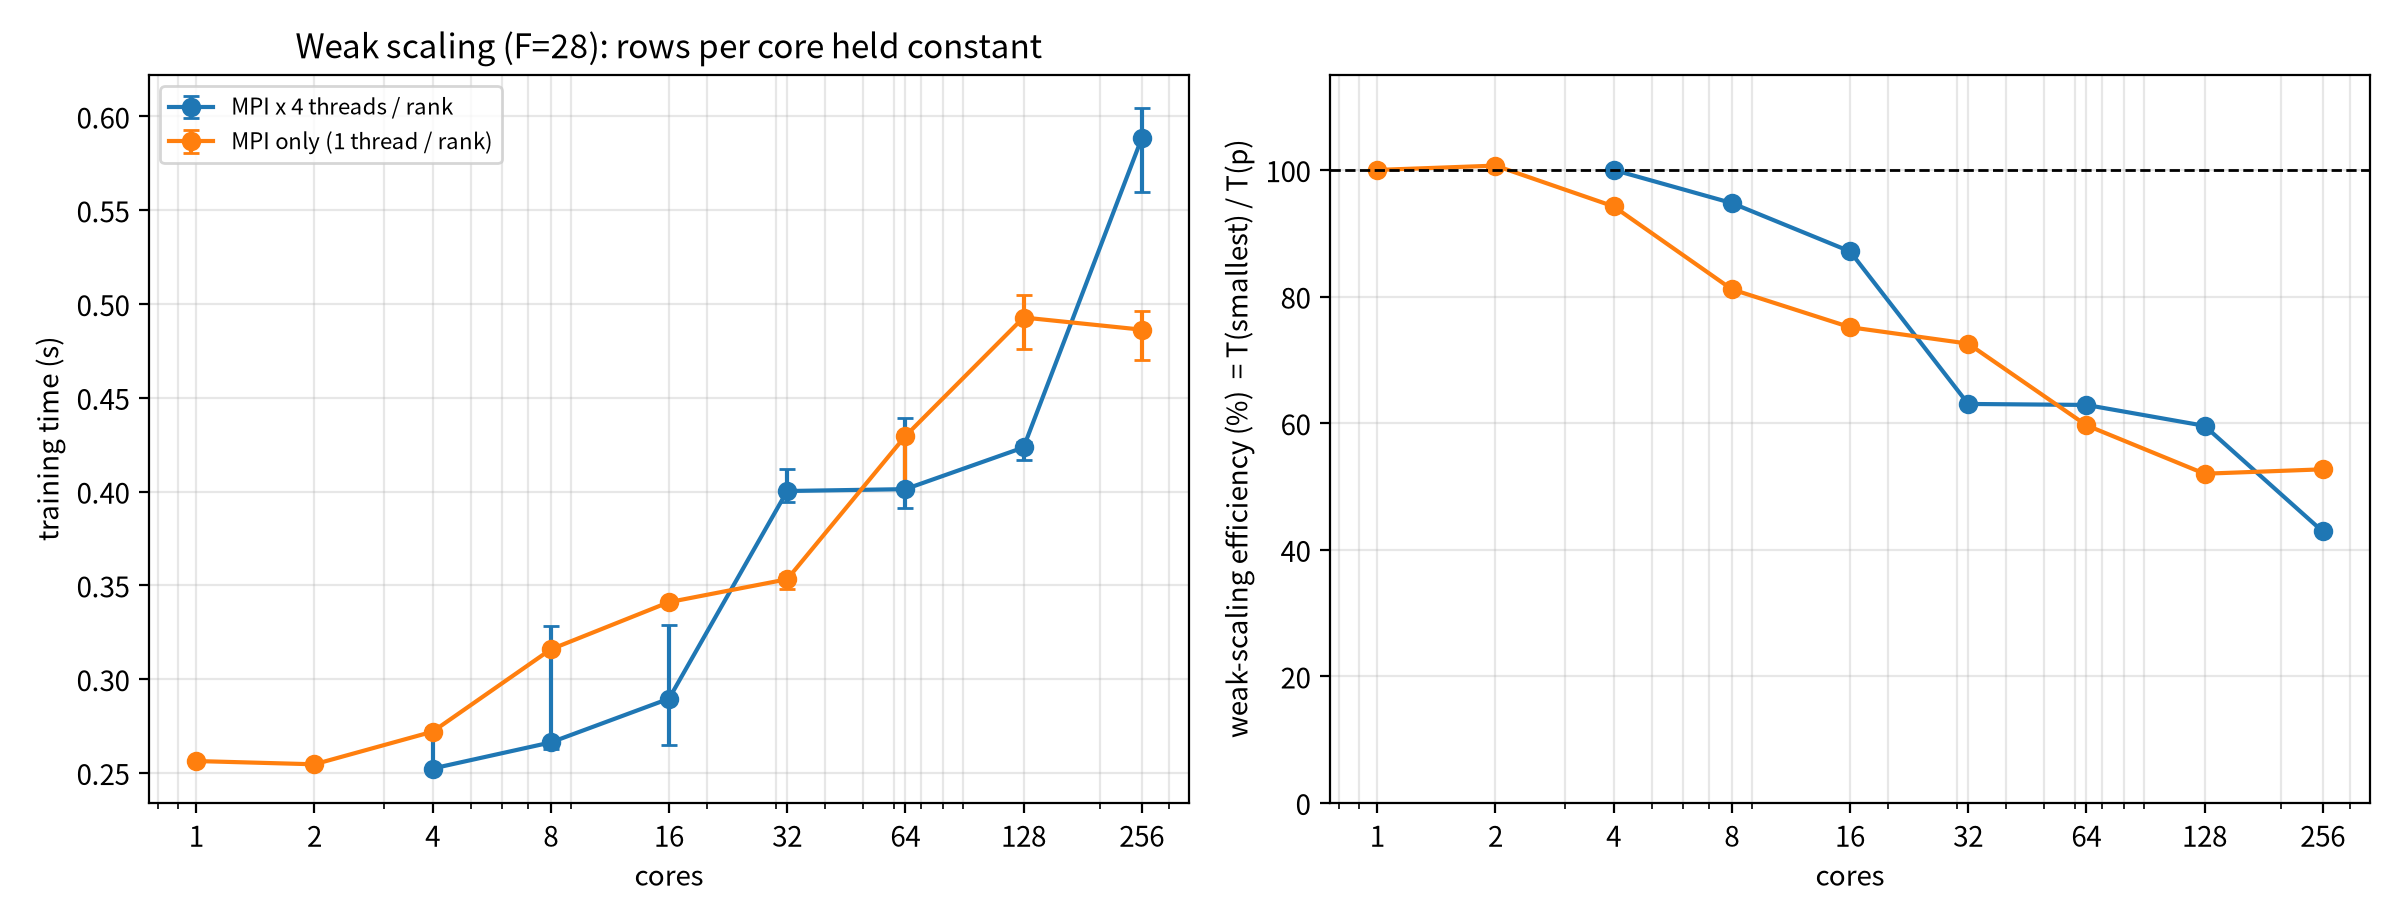
\includegraphics[width=\linewidth]{weak_scaling_F28.png}
\caption{Weak scaling runtime (left) and efficiency (right) at \num{1000000} rows/core up to \num{256} cores (\num{256}M rows, $F=\num{28}$) on Vanda.}
\label{fig:weak}
\end{figure}

Table~\ref{tab:weak} and Figure~\ref{fig:weak} show that scaling problem size \num{256}-fold (from \num{1}M to \num{256}M rows across four nodes) increases pure-MPI wall time by less than $1.9\times$ (\SI{0.256}{s} to \SI{0.486}{s}), sustaining \textbf{\SI{52.7}{\percent} weak scaling efficiency} at \num{256} cores (\SI{57.2}{\percent} at $F=7$, \SI{64.3}{\percent} at $F=14$, and \SI{54.4}{\percent} at $F=56$). Because per-core compute work is constant, the gradual drop from \num{8} to \num{64} cores reflects shared memory-bandwidth contention within a 64-core node, while the step beyond \num{64} cores reflects inter-node collective communication.

\subsection{The impact of communication}

With \texttt{--profile}, a barrier before each reduction separates time spent \emph{waiting} for the slowest rank (load imbalance) from time spent in the reduction itself (transfer). Figure~\ref{fig:breakdown} and Table~\ref{tab:breakdown} decompose the profiled $F=\num{56}$ strong-scaling runs into histogram build ($t_{\text{hist}}$), split scan ($t_{\text{scan}}$), row partition ($t_{\text{part}}$), barrier wait ($t_{\text{wait}}$) and \texttt{MPI\_Allreduce} transfer ($t_{\text{allreduce}}$).

\begin{table}[H]
\centering
\caption{Profiled runtime breakdown for pure MPI ($N=\num{32000000}, F=\num{56}$, depth \num{6}; from \texttt{strong\_breakdown.csv}).}
\label{tab:breakdown}
\begin{tabular}{rrrrrrr}
\toprule
Cores $p$ & $t_{\text{total}}$ (s) & $t_{\text{hist}}$ (s) & $t_{\text{part}}$ (s) & $t_{\text{wait}}$ (s) & $t_{\text{allreduce}}$ (s) & Comm + wait share \\
\midrule
  1 & 10.570 & 9.092 & 1.466 & 0.0000 & 0.0000 &  0.0\% \\
  8 &  1.468 & 1.244 & 0.193 & 0.0258 & 0.0029 &  2.0\% \\
 32 &  0.556 & 0.459 & 0.056 & 0.0319 & 0.0077 &  7.1\% \\
 64 &  0.293 & 0.219 & 0.029 & 0.0176 & 0.0256 & 14.7\% \\
128 &  0.182 & 0.123 & 0.015 & 0.0124 & 0.0300 & 23.3\% \\
256 &  0.098 & 0.060 & 0.008 & 0.0138 & 0.0148 & \textbf{29.2\%} \\
\bottomrule
\end{tabular}
\end{table}

\begin{figure}[H]
\centering
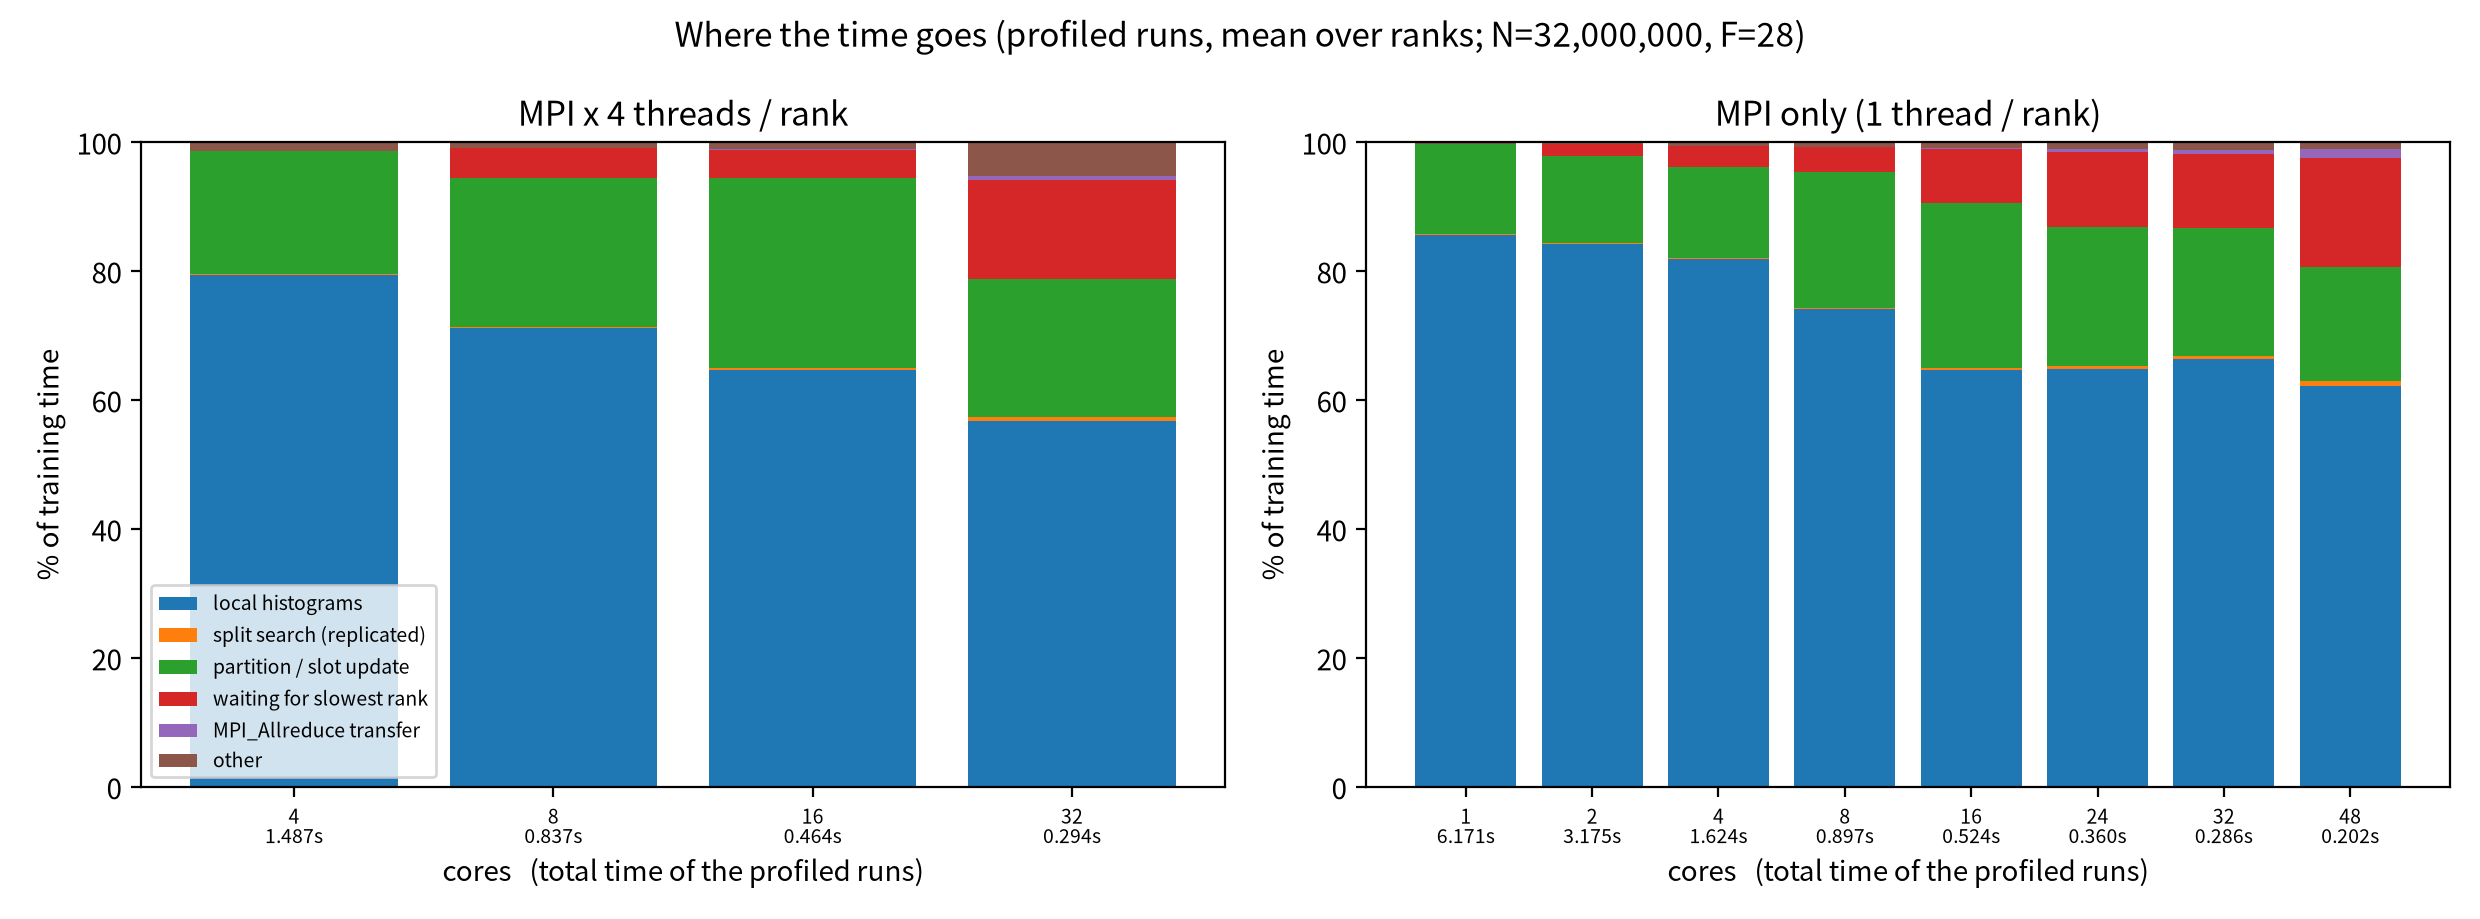
\includegraphics[width=\linewidth]{strong_breakdown.png}
\caption{Stacked phase breakdown vs.\ core count on Vanda ($N=\num{32000000}, F=\num{56}$): $t_{\text{hist}}$ and $t_{\text{part}}$ shrink as $O(1/p)$ while $t_{\text{wait}} + t_{\text{allreduce}}$ grows to \SI{29.2}{\percent} of runtime at \num{256} cores.}
\label{fig:breakdown}
\end{figure}

At $p=1$, histogram construction (\SI{86.0}{\percent}) and partitioning (\SI{13.9}{\percent}) account for \SI{99.9}{\percent} of the runtime. Both parallel phases shrink nearly ideally with $p$: from \num{1} to \num{256} cores, $t_{\text{hist}}$ drops \num{152}$\times$ (\SI{9.092}{s} $\to$ \SI{0.060}{s}) and $t_{\text{part}}$ drops \num{188}$\times$ (\SI{1.466}{s} $\to$ \SI{0.0078}{s}). In contrast, synchronization wait and \texttt{MPI\_Allreduce} transfer grow from \SI{2.0}{\percent} at \num{8} cores to \SI{14.7}{\percent} at \num{64} cores and \textbf{\SI{29.2}{\percent}} (\SI{28.6}{ms} out of \SI{98.0}{ms}) at \num{256} cores across four nodes, explaining why strong-scaling efficiency settles around \SI{30}{\percent}--\SI{37}{\percent} at \num{256} cores.

% ===========================================================================
\section{MPI+X: OpenMP hybrid and the GPU}\label{sec:mpix}
% [R4 10pt] MPI+X analysis; X=OpenMP => must also test on >=1 GPU

\subsection{MPI + OpenMP}

Adding OpenMP threads within each rank reduces the number of ranks sharing the reduction while keeping the cores busy. At a fixed total budget of \num{256} cores ($N=\num{32000000}, F=\num{28}$), we sweep the $\text{ranks}\times\text{threads}$ split from $256\times 1$ to $4\times 64$ (Table~\ref{tab:hybrid} and Figure~\ref{fig:hybrid}).

\begin{table}[H]
\centering
\caption{Runtime at fixed \num{256} cores across $\text{ranks}\times\text{threads}$ splits ($N=\num{32000000}, F=\num{28}$; from \texttt{hybrid\_fixed.csv}).}
\label{tab:hybrid}
\begin{tabular}{rrrrr}
\toprule
Ranks $\times$ Threads & Total cores & Median $T$ (s) & Min $T$ (s) & Max $T$ (s) \\
\midrule
$256 \times 1$  & 256 & 0.0686 & 0.0681 & 0.0687 \\
$128 \times 2$  & 256 & 0.0689 & 0.0679 & 0.0718 \\
$64 \times 4$   & 256 & 0.0693 & 0.0678 & 0.0694 \\
$32 \times 8$   & 256 & 0.0649 & 0.0648 & 0.0671 \\
$16 \times 16$  & 256 & 0.0721 & 0.0719 & 0.0737 \\
$8 \times 32$   & 256 & 0.0528 & 0.0526 & 0.0591 \\
$4 \times 64$   & 256 & \textbf{0.0479} & \textbf{0.0478} & 0.0574 \\
\bottomrule
\end{tabular}
\end{table}

\begin{figure}[H]
\centering
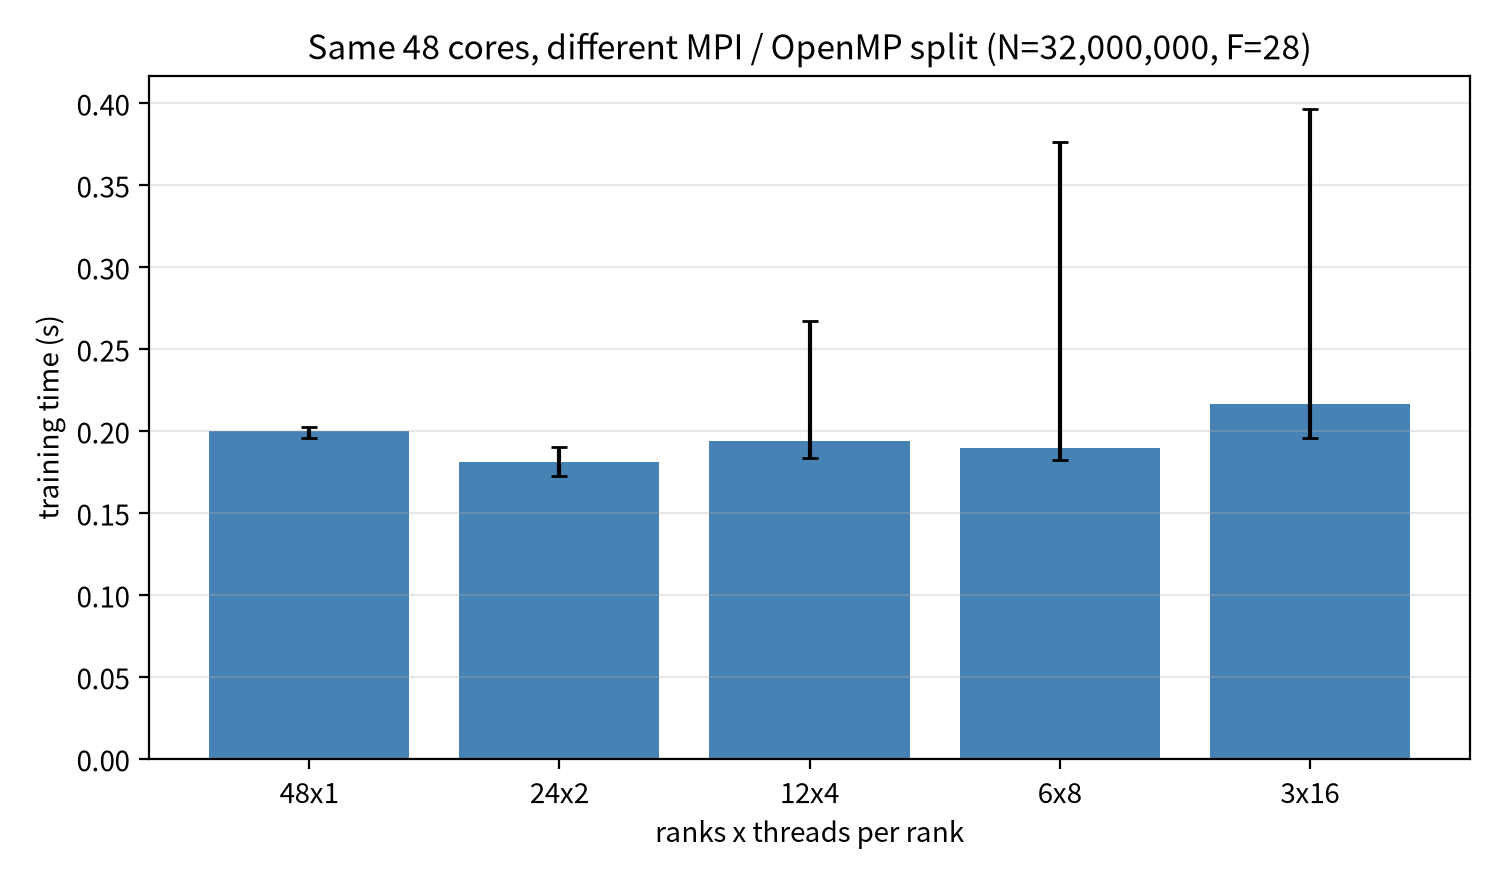
\includegraphics[width=0.78\linewidth]{hybrid_fixed_cores.png}
\caption{Fixed \num{256}-core runtime across MPI $\times$ OpenMP splits on Vanda ($N=\num{32000000}, F=\num{28}$).}
\label{fig:hybrid}
\end{figure}

Across \num{1} to \num{8} threads per rank ($256\times 1$ through $32\times 8$), median runtime is nearly flat (\SI{0.0649}{s}--\SI{0.0693}{s}), while one rank per socket ($8\times 32$, \SI{0.0528}{s}) and one rank per node ($4\times 64$, \textbf{\SI{0.0479}{s}}, or \num{107.9}$\times$ faster than serial) achieve the fastest times at \num{256} cores. With $4\times 64$, the inter-node \texttt{MPI\_Allreduce} involves only \num{4} processes instead of \num{256}, slashing collective communication overhead while OpenMP's thread-local histogram reduction aggregates counts in shared L3 cache within each node. Conversely, in the single-node strong-scaling sweep (\texttt{strong\_thr}), pure OpenMP on one node reaches \SI{0.219}{s} (\num{23.6}$\times$) at \num{64} threads versus \SI{0.202}{s} (\num{25.6}$\times$) for pure MPI, because thread-private histogram reduction across dual sockets incurs NUMA traffic when there is no inter-node MPI latency to save.

\subsection{CUDA on a GPU}
% required because X = OpenMP

Because the chosen X is OpenMP, we additionally implement the histogram hot path on a GPU in CUDA (\texttt{src/tree\_cuda.cu}) and benchmark it on a Vanda \textbf{NVIDIA A40} GPU. The kernel builds the exact same $F\times 256\times 2$ integer $[\text{count},\text{positive count}]$ histogram as the CPU, using thread-block shared-memory privatization followed by global atomic accumulation and a parallel split-scan kernel, so the split chosen matches the CPU result identically.

\begin{table}[H]
\centering
\caption{NVIDIA A40 GPU vs.\ CPU histogram and root-split benchmark on Vanda ($F=\num{28}$; from \texttt{gpu\_20261110\_214122\_1536934.csv} and \texttt{gpu\_20261110\_235027\_1537453.csv}).}
\label{tab:gpu}
\begin{tabular}{lrrrrr}
\toprule
Dataset size & CPU 1-core hist & A40 H2D transfer & A40 kernel + scan & A40 total & Compute / Total speedup \\
\midrule
$N=\num{2000000}, F=28$  & \SI{0.3778}{s} & \SI{0.00542}{s} & \SI{0.00586}{s} & \SI{0.01128}{s} & \textbf{64.44$\times$} / \textbf{40.61$\times$} \\
$N=\num{32000000}, F=28$ & \SI{0.6041}{s} & \SI{0.08557}{s} & \SI{0.09346}{s} & \SI{0.17905}{s} & \textbf{6.46$\times$} / \textbf{4.13$\times$} \\
\bottomrule
\end{tabular}
\end{table}

Table~\ref{tab:gpu} reports both benchmark sizes:
\begin{itemize}
  \item At $N=\num{2000000}, F=\num{28}$, the NVIDIA A40 builds the histogram and finds the root split in \textbf{\SI{5.86}{ms}} of kernel time (\SI{11.28}{ms} including the \SI{5.42}{ms} PCIe host-to-device copy), achieving a \textbf{\num{64.44}$\times$ compute speedup} and \textbf{\num{40.61}$\times$ end-to-end speedup} over one CPU core (\SI{0.3778}{s} histogram, \SI{0.4580}{s} total). Both select feature \num{4}, threshold \num{3.5}, with Gini gain \num{0.016713}.
  \item At $N=\num{32000000}, F=\num{28}$ (\num{1380} non-empty feature bins, \SI{896}{MB} of uint8 feature data plus labels), the A40 kernel runs in \textbf{\SI{93.46}{ms}} and the PCIe Gen4 host-to-device transfer takes \SI{85.57}{ms} (\SI{10.47}{GB/s}), for an end-to-end GPU time of \SI{0.1791}{s} versus \SI{0.6041}{s} CPU histogram time (\SI{0.7390}{s} total depth-1 time) on one core --- a \num{6.46}$\times$ kernel speedup (\num{4.13}$\times$ including PCIe transfer), and matching a 4-core OpenMP node on the root pass. Both CPU and GPU choose the exact same split: feature \num{4}, threshold \num{3.5}, Gini gain \num{0.016735}.
\end{itemize}

% ===========================================================================
\section{Discussion and conclusions}\label{sec:discuss}
% [R5 5pt] overall discussion + real-data conclusions

\paragraph{How the problem was parallelized.}
Our implementation distributes rows statically across MPI ranks and represents each candidate split via exact integer histograms. Because histogram entries are additive integers, a single collective \texttt{MPI\_Allreduce} per tree level suffices to give every rank the global class counts, guaranteeing bit-for-bit identical trees across serial, MPI, and OpenMP runs. Growing the tree level-wise batches all active nodes at a given depth into one reduction (\num{7} collectives instead of \num{64} at depth \num{6}, giving a \num{2.73}$\times$ speedup at \num{256} cores), while row-parallel OpenMP threads within each rank reduce MPI communicator size and network contention. On the GPU, shared-memory histogram privatization yields up to \num{64.4}$\times$ kernel speedup over a single CPU core. As the profiled breakdown in Section~\ref{sec:mpi} demonstrates, local histogram construction scales as $O(N/p)$ and shrinks by \num{152}$\times$ at \num{256} cores, leaving inter-node \texttt{MPI\_Allreduce} latency and synchronization wait (\SI{29.2}{\percent} of runtime at \num{256} cores) as the primary scaling limit.

\paragraph{Conclusions about the data.}
On \texttt{instacart\_clean.csv} ($N=\num{200000}, F=\num{7}$) the serial tree reaches \textbf{\SI{68.50}{\percent}} training accuracy at depth \num{6}, against a majority-class baseline of \SI{66.17}{\percent} (\num{67669} of \num{200000} rows, or \SI{33.83}{\percent}, are reorders), a modest but consistent improvement that matches scikit-learn to \SI{99.985}{\percent} prediction agreement. Inspecting \texttt{--dump-tree} shows that the root split is \texttt{add\_to\_cart\_order} $\le 3.5$ (feature \num{4}), immediately separating staple items placed into the cart first from later additions, while the next levels split on \texttt{days\_since\_prior\_order} around $6.5$--$9.5$ days (feature \num{3}, capturing weekly replenishment cycles), \texttt{order\_number} (feature \num{0}), and \texttt{aisle\_id} (feature \num{5}). Finally, Figure~\ref{fig:real} shows why scaling studies require synthetic data: on \num{200000} rows, serial training takes only \SI{24.1}{ms}, reaches a minimum of \textbf{\SI{1.69}{ms}} at \num{32} cores (\num{14.25}$\times$ speedup), and then slows down at \num{64}--\num{256} cores (\SI{5.61}{ms} at \num{256} cores) because each rank holds only \num{781} rows and inter-node \texttt{MPI\_Allreduce} latency completely dominates computation.

\begin{figure}[H]
\centering
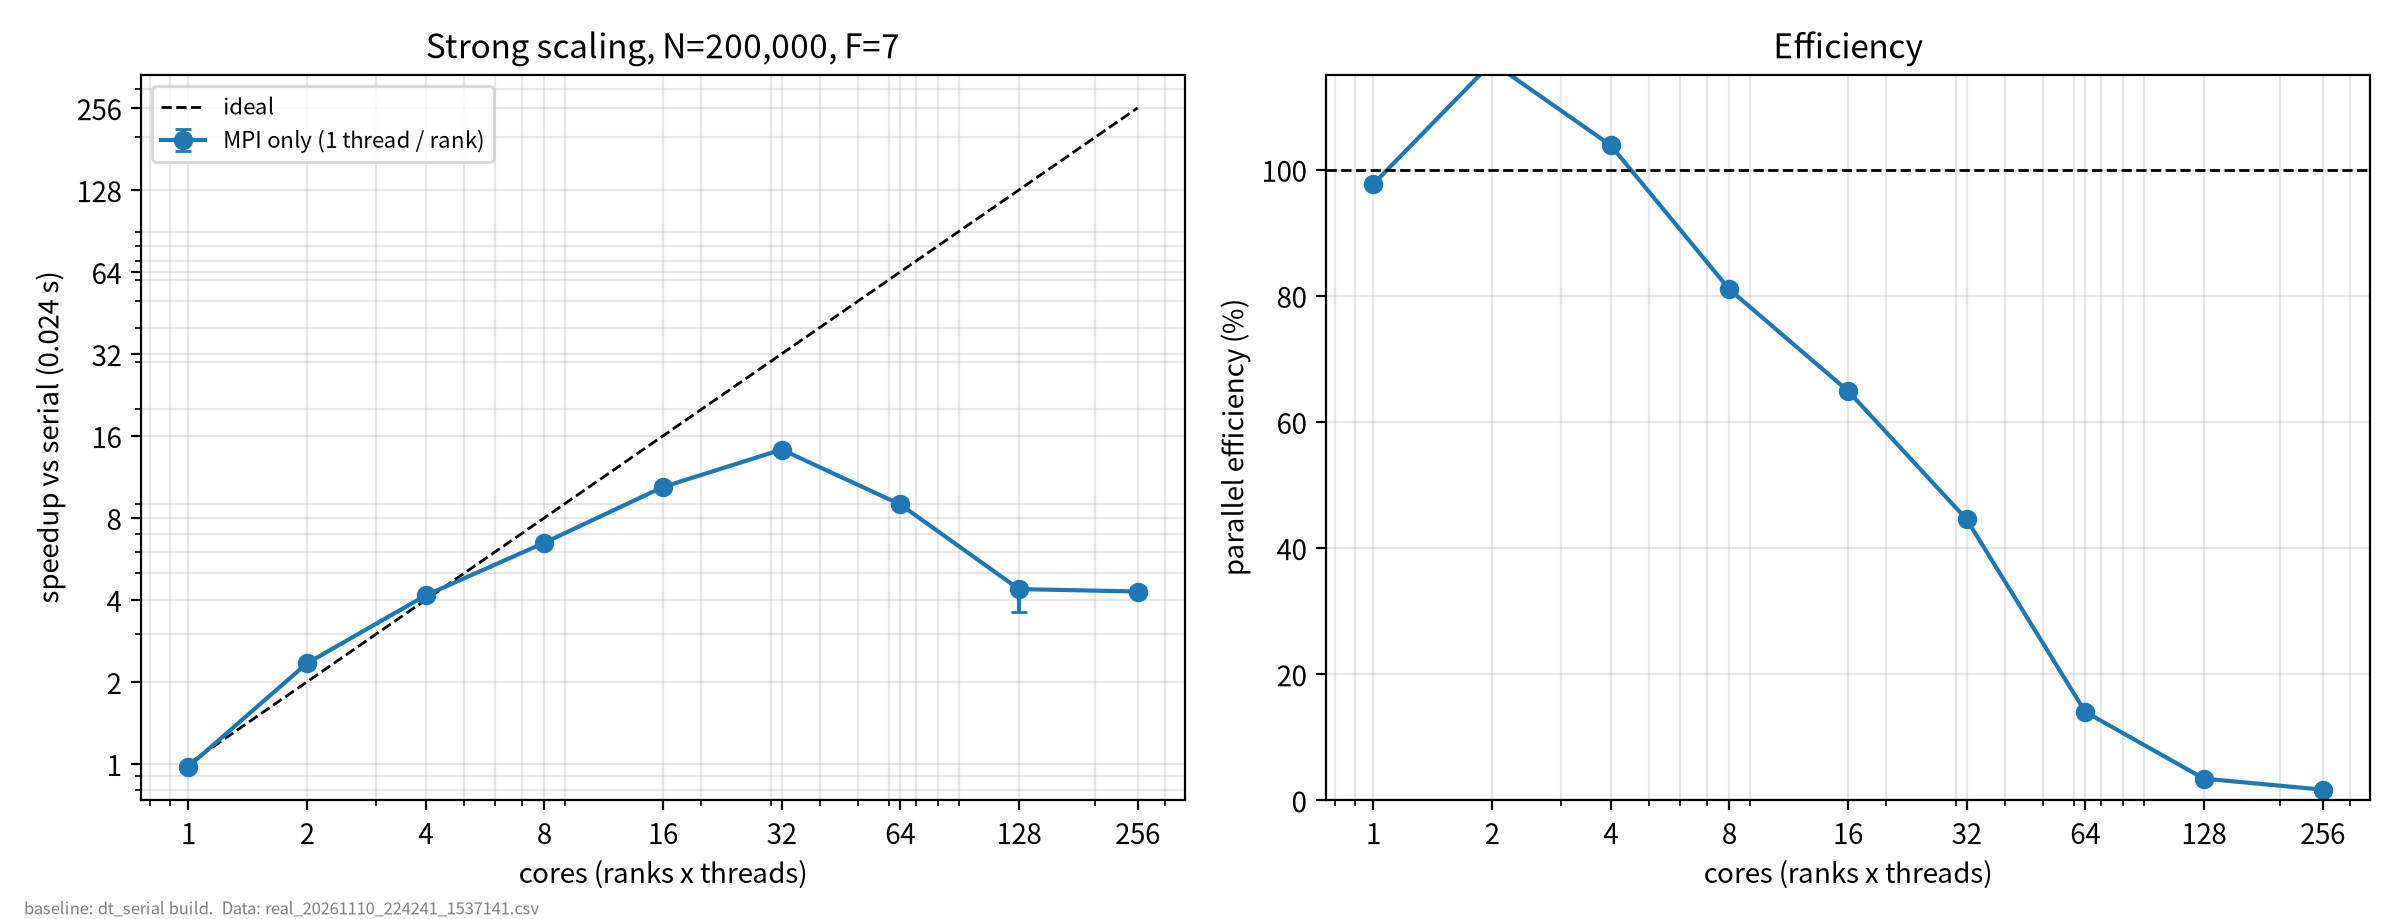
\includegraphics[width=0.85\linewidth]{real_scaling.png}
\caption{Strong scaling on the \num{200000}-row \texttt{instacart\_clean.csv} dataset on Vanda: runtime bottoms out at \SI{1.69}{ms} (\num{32} cores, \num{14.25}$\times$ speedup) before collective latency dominates.}
\label{fig:real}
\end{figure}

% ===========================================================================
\section{AI usage}\label{sec:ai}
% general instruction: explanation of any AI usage

Anthropic's Claude (via the Claude Code CLI) and Google's Gemini (via Antigravity) assisted with code review, with diagnosing the earlier MPI split-search correctness issue, with PBS batch script troubleshooting, and with drafting and structuring this report. All design decisions, the choice of algorithm and parallelization strategy, and the final analysis were the authors'. All AI-assisted code was reviewed, compiled and run by the authors, and every reported number comes from an actual run on the NUS Vanda HPC cluster.

\end{document}
